\section{\color{blue} Effect of Second Reverse Edge on the Consensus of Double Integrators}
%%%%%%%%%%%%%%%%%%%%%%%%%%%%%%%%%%%%%%%%%%%%%%%%%%%%%
%\begin{frame}[noframenumbering]
%	\tableofcontents[currentsection]
%\end{frame}
%%%%%%%%%%%%%%%%%%%%%%%%%%%%%%%%%%%%%%%%%%%%%%%%%%%%
\begin{frame}
	%\centering
	\textcolor{blue}{Approach 1:} Can we add another cycle in the network to reduce or remove this bound?\\ 
	%\pause
	\vspace{-0.2cm}
	%There are 6 different cases of the second cycle interaction in the said network topology. 
	%Let $\mathcal{V}_1,\mathcal{E}_1$ be the node and edge set of first cycle and $\mathcal{V}_2,\mathcal{E}_2$ be the node and edge set of the second cycle. \vspace{-0.5cm} %Let the characteristic equation be represented by polynomial $p(s)$, where $s=1-\lambda$ and $\lambda$ are the eigenvalues of the matrix $\mathcal{C}$\\
	\begin{figure}
		\centering
		\subfloat[]%t[$\mathcal{V}_1 \cap \mathcal{V}_2=\phi,\mathcal{E}_1 \cap \mathcal{E}_2=\phi$]
		{
			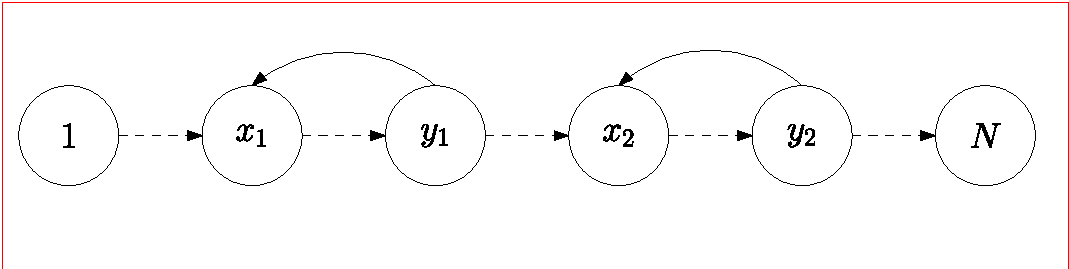
\includegraphics[width=0.35\textwidth,keepaspectratio]{Images/Fig1.pdf}
		}
		\subfloat[]%[$\mathcal{V}_1 \cap \mathcal{V}_2\neq \phi,\mathcal{E}_1 \cap \mathcal{E}_2=\phi$]
		{
			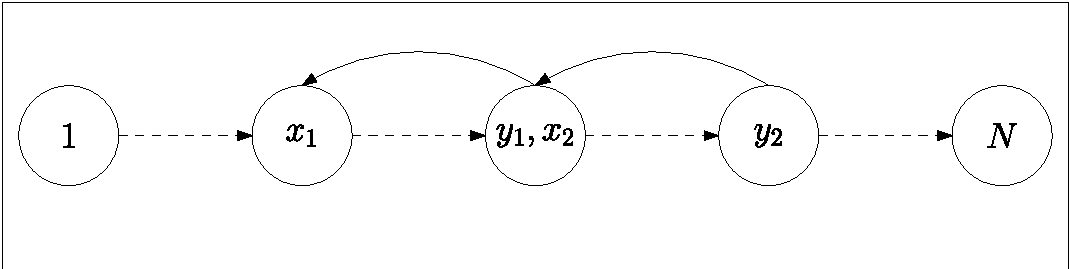
\includegraphics[width=0.35\textwidth,keepaspectratio]{Images/Fig2.pdf}
		}
		\vspace{-3mm}
		\subfloat[]%[$\mathcal{V}_2 \not\subset \mathcal{V}_1,\mathcal{E}_1 \cap \mathcal{E}_2 \neq \phi$]
		{
			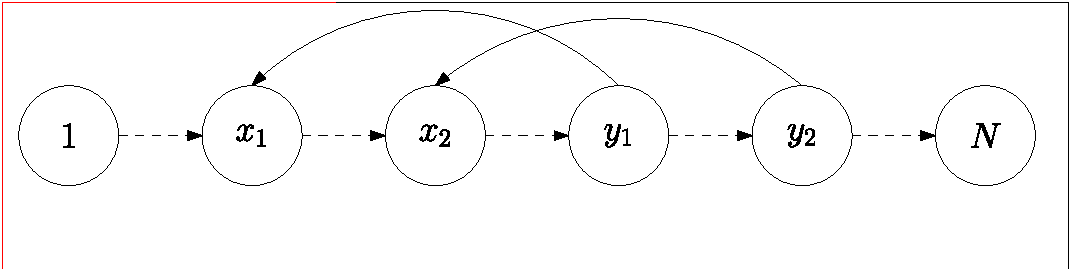
\includegraphics[width=0.35\textwidth,keepaspectratio]{Images/Fig3.pdf}
		}
		\subfloat[]%[$\mathcal{V}_2 \subset \mathcal{V}_1,\mathcal{E}_1 \cap \mathcal{E}_2 \neq \phi,y_2 \neq y_1,x_2 \neq x_1$]
		{
			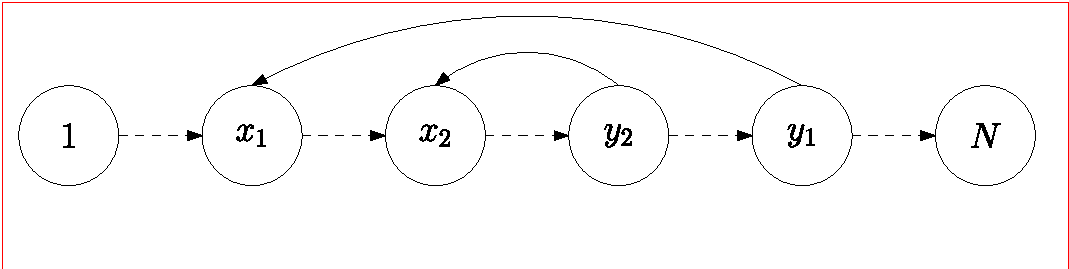
\includegraphics[width=0.35\textwidth,keepaspectratio]{Images/Fig4.pdf}
		}
		\vspace{-3mm}
		\subfloat[]%[$\mathcal{V}_2 \subset \mathcal{V}_1,\mathcal{E}_1 \cap \mathcal{E}_2 \neq \phi,y_2=y_1,x_2 \neq x_1$]
		{
			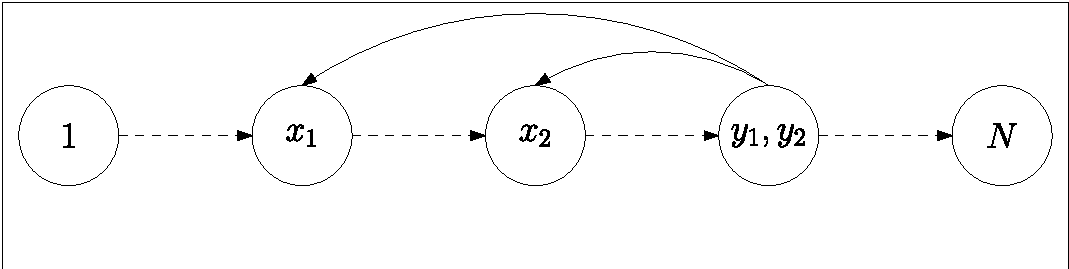
\includegraphics[width=0.35\textwidth,keepaspectratio]{Images/Fig5.pdf}
		}
		\subfloat[]%[$\mathcal{V}_2 \subset \mathcal{V}_1,\mathcal{E}_1 \cap \mathcal{E}_2 \neq \phi,y_2 \neq y_1,x_2=x_1$]
		{
			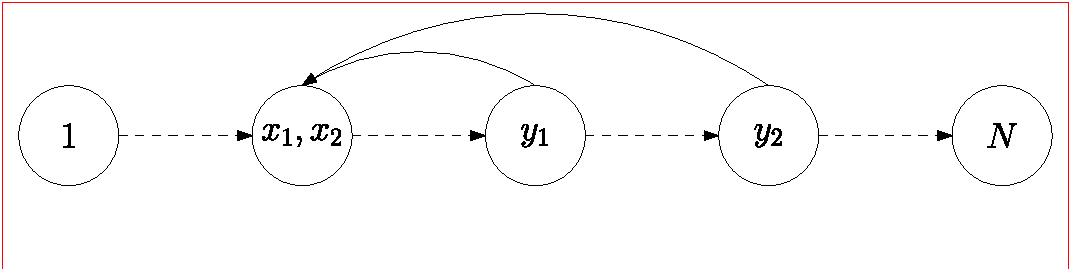
\includegraphics[width=0.35\textwidth,keepaspectratio]{Images/Fig6.pdf}
		}
		\vspace{-2mm}
		%\caption{Different Case of Two reverse Edge Interactions in a chain network}
	\end{figure}
	%\vspace{-0.5cm}
	%\pause
	\textbf{Note 1:} Red boxes indicates similar work by other researchers but in context to single integrators\footnotemark[1]$^,$\footnotemark[2]
	\vspace{0.1cm}
	\footnotetext[1]{\textcolor{blue}{Hao Y, Wang Q, Duan Z,Chen G}, {\em The role of reverse edges on consensus performance of chain networks}, IEEE Transactions on Systems, Man, and Cybernetics: Systems 2019.}
	\footnotetext[2]{\textcolor{blue}{H. -T. Zhang, Z. Chen and X. Mo}, {\em Effect of Adding Edges to Consensus Networks With Directed Acyclic Graphs}, IEEE Transactions on Automatic Control, 2017.}.\\
%	\textbf{Note 2:} Fig. (a)-(c) can be further divided in three sub-cases (i)$l_1>l_2$,(ii)$l_1<l_2$ and (iii) $l_1 = l_2$.\\
	%\textbf{Note 3:} The claims~\footnotemark[1] would be incorrect if the condition in \textbf{Note 2} is not specified.
	
	%\alt<1>{\let\thefootnote\relax\footnotetext{~}}{\footnotetext[1]{\textcolor{blue}{Hao Y, Wang Q, Duan Z,Chen G}, {\em The role of reverse edges on consensus performance of chain networks}, IEEE Transactions on Systems, Man, and Cybernetics: Systems 2019.}}
	%\alt<1>{\let\thefootnote\relax\footnotetext{~}}{\footnotetext[2]{\textcolor{blue}{H. -T. Zhang, Z. Chen and X. Mo}, {\em Effect of Adding Edges to Consensus Networks With Directed Acyclic Graphs}, IEEE Transactions on Automatic Control, 2017.}}
\end{frame}


\begin{subframe}
	The $\gamma$ bound is characterized by the eigenvalues of matrix $\mathcal{C}$ captured in the Laplacian matrix by the reverse edge addition as:\\
	%\centering
	$$\mathcal{L}=\begin{bmatrix}
		\mathcal{L}_1 & 0 & 0 \\
		* & \mathcal{C} & 0 \\
		* & * & \mathcal{L}_2
	\end{bmatrix} \text{ (without Leader)}$$ 
	\vspace{0.2cm}
	Let the characteristic equation of the matrix $\mathcal{C}$ be represented by the polynomial $$\chi(s)=p(s)-1,$$ where $s=1-\lambda$ and $\lambda$ are the eigenvalues of the matrix $\mathcal{C}$\\
	\vspace{-0.2cm}
	%\pause
	%\begin{block} {Polynomial Equations}
	%Then the polynomial equation p(s) will take either one of the form:
	%\begin{enumerate}
	%	\item %\begin{equation} \label{Polynomial1}
	%$p(s,l_2)=s^{l_2+2}+2s^{l_2+1}+s^{l_2}-2s=1, l_2 \in \mathbb{N} \text{ and }l_2 \geq 1$.
	%\end{equation}
	%with $l_2 \in \mathbb{N}$ and $l_2 \geq 1$.
	%\item %\begin{equation} \label{Polynomial2}
	%	$p(s,l_1,l_2)=s^{l_2+2}+2s^{l_2+1}+s^{l_2}-s^{l_2-l_1+1}-s=1, l_2,l_1 \in \mathbb{N}\text{ and }l_2>l_1 \geq 1.$
	%\end{equation}
	%with $l_2,l_1 \in \mathbb{N}$ and $l_2>l_1 \geq 1$.
	%\item %\begin{equation} \label{Polynomial3}
	%$p(s,l_1,l_2)=s^{l_1}(s+2)-s^{l_1-l_2}=1, l_2,l_1 \in \mathbb{N}\text{ and }l_1>l_2 \geq 1.$
	%\end{equation}
	%with $l_2,l_1 \in \mathbb{N}$ and $l_1>l_2 \geq 1$.
	%\item %\begin{equation} \label{Polynomial4}
	%$p(s,l_1,l_2)=s^{l_1+1}+2s^{l_1}+s^{l_1-1}-s^{l_1-l_2}-s^{l_1-l_2-1}=1, l_2,l_1 \in \mathbb{N}\text{ and }l_1>l_2 \geq 1.$
	%\end{equation}
	%with $l_2,l_1 \in \mathbb{N}$ and $l_1>l_2 \geq 1$.
	%\item %\begin{equation} \label{Polynomial5}
	%$p(s,l_1,l_2)=s^{l_i+1}+s^{l_i}=1, l_i=\max(l_1,l_2).$
	%\end{equation}
	%with $l_i=\max(l_1,l_2)$
	%\end{enumerate}
	%\pause
	The following statements are always true for equation p(s):
	\begin{enumerate}
		\item It has only one real solution between (0,1) say $s_1$.
		\item Real parts of other roots are smaller than $s_1$.
		\item $s_1$ is a strictly increasing function of $l_2$.
	\end{enumerate}
	\hyperlink{BetterSuff}{\beamerbutton{Back}}~~\hyperlink{Conc:Approach1}{\beamerbutton{Approach1}}
\end{subframe}


%\pause
\begin{comment}
	\begin{block}{Theorem 1}
		Consensus among double integrators, described by \eqref{SecondConsensus}, is achieved asymptotically if the networked system has a directed spanning tree and \\
		\begin{equation}\label{new-sufficiency}
			\gamma \geq \frac{1}{\sqrt{1-s_1}}=\frac{1}{\sqrt{\lambda_1}} \text{  \bigg(Better Sufficient Condition, \textcolor{red}{Earlier $\frac{2}{\sqrt{\lambda_1}}$}\bigg)}
		\end{equation}	
		where $s_1$ is the real solution of the relevant polynomial equations p(s) and $\lambda_1$ is the corresponding eigenvalue of the matrix $\mathcal{C}$ based on lengths of directed cycle and the interaction among the two cycles.
	\end{block}	
\end{comment}
%\end{block}


\begin{subframe}
	\vspace{-0.1cm}
	\begin{theorem}[Better Sufficiency Condition]\label{BetterSuff}
		Consensus among double integrators is achieved asymptotically if the networked system has a directed spanning tree and \\
		\begin{equation*}\label{new-sufficiency}
			\gamma \geq \frac{1}{\sqrt{1-s_1}}=\frac{1}{\sqrt{\lambda_1}} \text{  \bigg(Better Sufficient Condition, \textcolor{red}{Earlier $\frac{2}{\sqrt{\lambda_1}}$}\bigg)}
		\end{equation*}	
		where $s_1$ is the real solution of the relevant polynomial equations p(s) and $\lambda_1$ is the corresponding eigenvalue of the matrix $\mathcal{C}$. %based on lengths of directed cycle and the interaction among the two cycles. 
		\hyperlink{LapStruct}{\beamerbutton{$\mathcal{C} Structure$}}
	\end{theorem}	
	\vspace{-0.2cm}
	\begin{theorem}[Effect of Cycle on Eigenvalues]
		A cycle of length $l$ on a directed chain of $N$ nodes affects $l$ eigenvalues of the Laplacian if such a cycle contains the root node, and affects $l+1$ eigenvalues otherwise.
	\end{theorem}
	\vspace{-0.2cm}
	\begin{block}{Conclusions}
		\begin{enumerate}
			\item Deduced better sufficiency condition
			\item Need not to search over the entire spectra but the knowledge of the only real root is sufficient.
			\item The lengths of cycle and their relative positions are sufficient for finding the bound and is independent of the network size. \hyperlink{Conc:Approach1}{\beamerbutton{Approach1}}
		\end{enumerate}
	\end{block}
	
\end{subframe}
